
Due to the difference in wordsize between the old and new communication unit, a compatibility layer is added to allow other existing code to remain unchanged.

\figurename~\ref{fig:overview-lundal} shows the changes to the hardware platform.
The old COM40 unit has been replaced by a new communication unit and a compatibility layer.
The compatibility layer is needed because the old COM40 unit was based on 64-bit data while PCI Express uses 32-bit data.
\todo{blergh}

\begin{figure}[!ht]
    \centering
    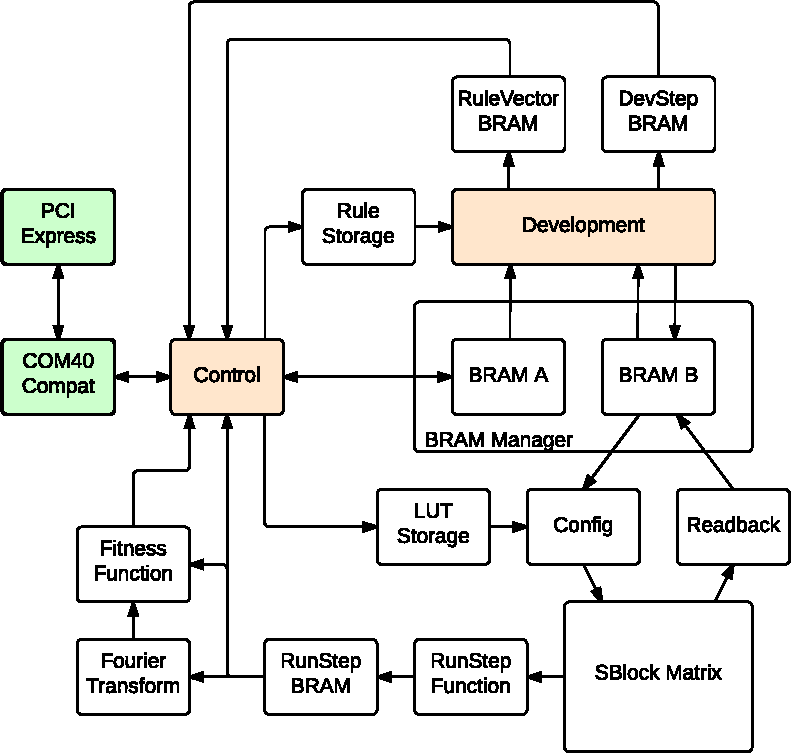
\includegraphics[width=0.48\textwidth]{figures/overview-lundal}
    \caption{High-level block diagram of the current hardware platform. Additions are highlighted in green.}
    \label{fig:overview-lundal}
\end{figure}

The communication unit has internal data buffers.

On the software side, the api uses linux' built-in drivers for PCI Express.

\subsection{Overview}

The new communication unit is based on Xilinx' reference PCI Express programmed io design.
It consists of the Xilinx PCI Express endpoint core, reception and transmission engines, data buffers, and a special request handler, as shown in \figurename~\ref{fig:details-communication}.

\begin{figure}[!ht]
    \centering
    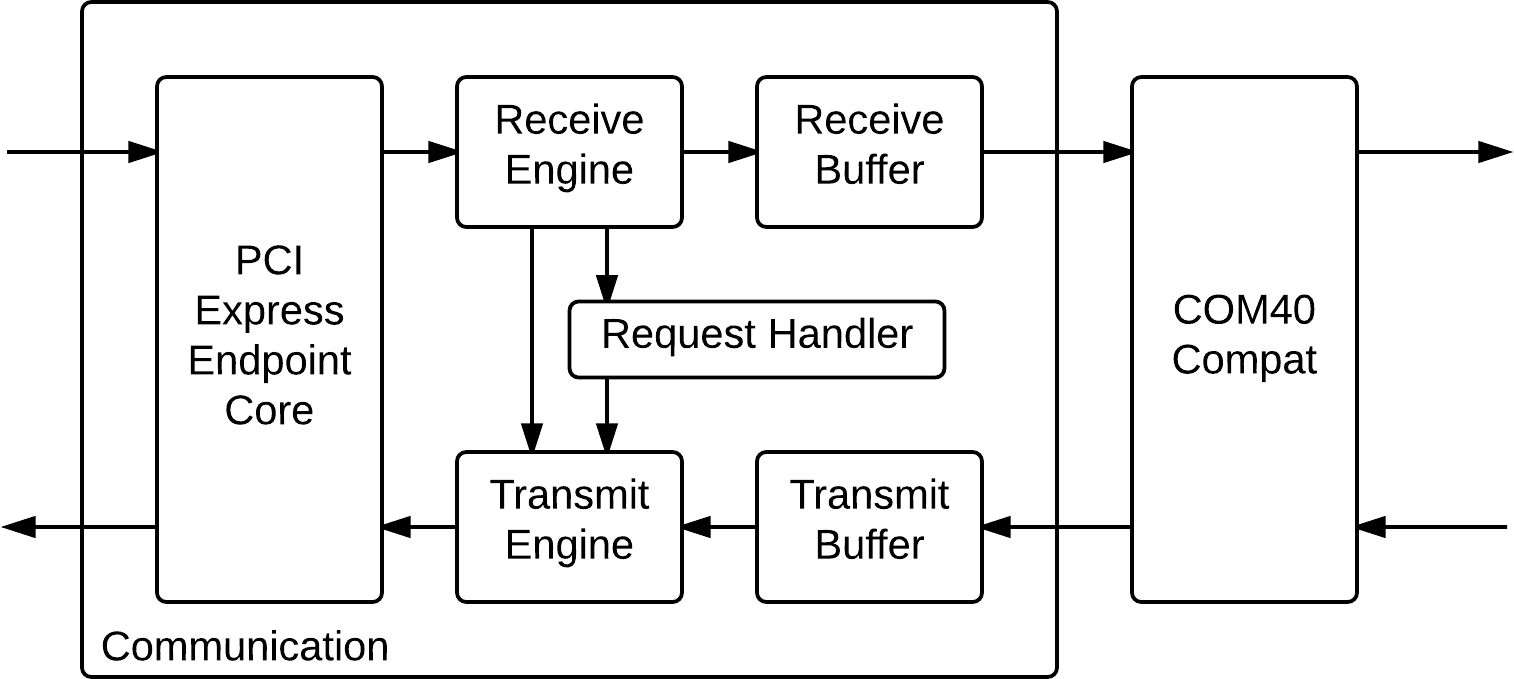
\includegraphics[width=0.48\textwidth]{figures/details-communication}
    \caption{Detailed block-diagram of the PCI Express communication module.}
    \label{fig:details-communication}
\end{figure}

The endpoint core completely handles the physical and data link layers, and all TLPs related to configuration and establishment of the PCI Express connection.
Other TLPs, such as read and write requests, are presented on an AXI4-Stream interface \cite{ug672}.
The reception engine is responsible for parsing TLPs and either writing received data to the reception buffer or notifying the transmission engine about a read request.
The transmission engine is responsible for building completer TLPs to respond to read requests, using data from the transmission buffer.
The request handler listens to the read requests provided by the reception engine, and can override the transmission engine to respond to special requests.

\subsection{PCI Express Endpoint Core}

\todo{bars, wrapper, id, more?}

\subsection{Reception engine}

The reception engine is implemented as a simple state machine, as shown in \figurename~\ref{fig:statemachine-receive}.

\begin{figure}[!ht]
    \centering
    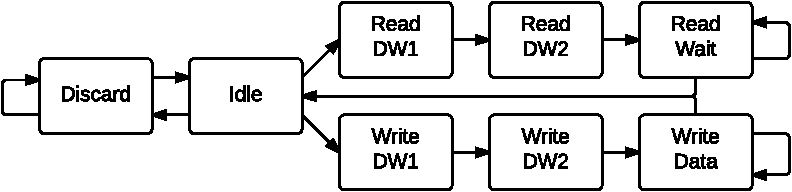
\includegraphics[width=0.48\textwidth]{figures/statemachine-receive}
    \caption{State machine for the reception engine.}
    \label{fig:statemachine-receive}
\end{figure}

Until the endpoint core presents valid data, the state machine remains in Idle.
When it does, the data is stored, and the TLP type is checked.
If it is a read or write request, the state machine continues down the corresponding path, otherwise the remaining data is discarded.
The remaining portion of the TLP headers are then parsed in the DW1 and DW2 states.
For read requests, the state machine waits in ReadWait until the transmission engine is ready to accept a new read request, and then proceeds to Idle.
For write requests, the state machine stays in WriteData, where one DW of data is written to the reception buffer each cycle, for the length of the packet, and then proceeds to Idle.

\subsection{Transmission engine}

The transmission engine is implemented as a simple state machine, as shown in \figurename~\ref{fig:statemachine-transmit}.

\begin{figure}[!ht]
    \centering
    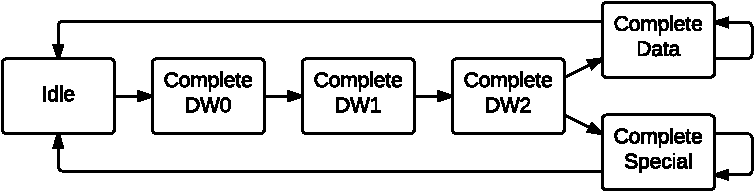
\includegraphics[width=0.48\textwidth]{figures/statemachine-transmit}
    \caption{State machine for the transmission engine.}
    \label{fig:statemachine-transmit}
\end{figure}

Until the reception engine signals a read request, the state machine remains in Idle.
When a read request is signaled by the reception engine, the state machine begins to traverse the DW path.
The DW0, DW1 and DW2 states each transmit one DW of the completer TLP header.
Then if the special request signal is set, it procceds to CompleteSpecial, where it transmits data presented by the request handler.
Otherwise, it proceeds to CompleteData where it transmits one DW of data from the transmission buffer each cycle.
When the requested number of DWs has been transmitted it proceeds back to Idle.

\subsection{Request handler}

The request handler continually listens to the read requests presented by the reception engine.
If the request is targeting the primary memory area (BAR 0), it is a normal read request and the transmission engine is allowed to proceed as usual.
Otherwise, it is a special request and the transmission engine is overridden.

The kind of special request is determined by the address of the read request, and handled thereafter.
There are currently four special requests implemented, as shown in Table~\ref{tab:requests}.

\begin{table}[!ht]
    \renewcommand{\arraystretch}{1.3}
    \caption{Special requests}
    \label{tab:requests}
    \centering
    \begin{tabular}{c|l}
        \bfseries Address & \bfseries Request \\
        \hline
        0x00 & Get transmission buffer data count \\
        0x01 & Get transmission buffer available space \\
        0x02 & Get reception buffer data count \\
        0x03 & Get reception buffer available space \\
    \end{tabular}
\end{table}

Note that each of the implemented special requests assumes a read request length of one DW.
If the request has a greater length, the returned data is simply repeated that number of times.

\subsection{Buffers}

\todo{describe fifo buffers}

\begin{figure}[!ht]
    \centering
    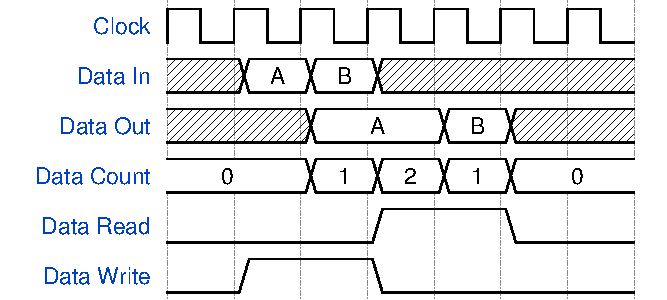
\includegraphics[width=0.40\textwidth]{figures/wavediagram-fifo}
    \caption{Wave diagram for the FIFO buffer, showing two consecutive writes followed by two consecutive reads.}
    \label{fig:wavediagram-fifo}
\end{figure}

Notice how the read signal needs to be asserted before the clock tick when data is read to ensure correct consecutive reads.
This is due to the BRAM used in the FIFO, which updates at clock ticks.
Therefore, the address has to be updated before the clock tick (by the read signal) to have correct data available for a read in the following cycle.

\subsection{Software API}

\todo{native linux driver, files under /sys/devices/pci}

